\documentclass[landscape,final,paperwidth=48in,paperheight=48in,fontscale=0.285]{baposter}
%\usepackage{calc,array}
\usepackage{graphicx} % Required for including images
\usepackage{amsmath}  % For typesetting math
\usepackage{amssymb}  % Adds new symbols to be used in math mode
\usepackage{relsize}  % Change size of text /smaller, /larger
\usepackage{multirow} % Allows table cells to span more than one row of the table
\usepackage{rotating} % Rotate figures and tables
\usepackage{bm}       % Allows a math expression to be bold
\usepackage{url}      % Allows email address and websites
\usepackage{gensymb}  % Allows degree symbol
\usepackage{siunitx}  % Scientific notation

\usepackage{float}
\usepackage{caption} % Required for specifying captions to tables and figures
\usepackage{wrapfig} % Wrap text around figure
\usepackage[export]{adjustbox}
\bibliography{IEEEabrv,poster_landscape}
%\captionsetup[figure]{font=Large,skip=0pt,labelformat=empty,justification=raggedright,singlelinecheck=false}

\usepackage{multicol} % Required for multiple columns

\usepackage[utf8]{inputenc} %Required for IEEE reference style
\newcommand{\BIBdecl}{\setlength{\itemsep}{-0.25 em}} %Removes line space between references

% Fonts
%\usepackage{times}
%\usepackage{helvet}
%\usepackage{bookman}
\usepackage{palatino}

%\newcommand{\captionfont}{\footnotesize}

\graphicspath{{/img}}
%\usetikzlibrary{calc}

\newcommand{\SET}[1]  {\ensuremath{\mathcal{#1}}}
\newcommand{\MAT}[1]  {\ensuremath{\boldsymbol{#1}}}
\newcommand{\VEC}[1]  {\ensuremath{\boldsymbol{#1}}}
\newcommand{\Video}{\SET{V}}
\newcommand{\video}{\VEC{f}}
\newcommand{\track}{x}
\newcommand{\Track}{\SET T}
\newcommand{\LMs}{\SET L}
\newcommand{\lm}{l}
\newcommand{\PosE}{\SET P}
\newcommand{\posE}{\VEC p}
\newcommand{\negE}{\VEC n}
\newcommand{\NegE}{\SET N}
\newcommand{\Occluded}{\SET O}
\newcommand{\occluded}{o}

%%%%%%%%%%%%%%%%%%%%%%%%%%%%%%%%%%%%%%%%%%%%%%%%%%%%%%%%%%%%%%%%%%%%%%%%%%%%%%%%
% Multicol Settings
%%%%%%%%%%%%%%%%%%%%%%%%%%%%%%%%%%%%%%%%%%%%%%%%%%%%%%%%%%%%%%%%%%%%%%%%%%%%%%%%
\setlength{\columnsep}{1.5em}
\setlength{\columnseprule}{0mm}
%%%%%%%%%%%%%%%%%%%%%%%%%%%%%%%%%%%%%%%%%%%%%%%%%%%%%%%%%%%%%%%%%%%%%%%%%%%%%%%%
% Save space in lists. Use this after the opening of the list
%%%%%%%%%%%%%%%%%%%%%%%%%%%%%%%%%%%%%%%%%%%%%%%%%%%%%%%%%%%%%%%%%%%%%%%%%%%%%%%%
\newcommand{\compresslist}{%
\setlength{\itemsep}{1pt}%
\setlength{\parskip}{0pt}%
\setlength{\parsep}{0pt}%
}
%%%%%%%%%%%%%%%%%%%%%%%%%%%%%%%%%%%%%%%%%%%%%%%%%%%%%%%%%%%%%%%%%%%%%%%%%%%%%%
%%% Begin of Document
%%%%%%%%%%%%%%%%%%%%%%%%%%%%%%%%%%%%%%%%%%%%%%%%%%%%%%%%%%%%%%%%%%%%%%%%%%%%%%

\begin{document}

%%%%%%%%%%%%%%%%%%%%%%%%%%%%%%%%%%%%%%%%%%%%%%%%%%%%%%%%%%%%%%%%%%%%%%%%%%%%%%
%%% Here starts the poster
%%%---------------------------------------------------------------------------
%%% Format it to your taste with the options
%%%%%%%%%%%%%%%%%%%%%%%%%%%%%%%%%%%%%%%%%%%%%%%%%%%%%%%%%%%%%%%%%%%%%%%%%%%%%%
% Define some colors

%\definecolor{lightblue}{cmyk}{0.83,0.24,0,0.12}
\definecolor{lightblue}{rgb}{0.145,0.6666,1}

%\newtcolorbox{demobox}[1][]{colback=white,colframe=lightblue,width=0.33\linewidth,nobeforeafter,box align=top,before=\noindent,#1}

%%
\begin{poster}%
  % Poster Options
  {
  % Show grid to help with alignment
  grid=false,
  % Column spacing
  colspacing=1em,
  % Color style
  bgColorOne=white,
  bgColorTwo=white,
  borderColor=lightblue,
  headerColorOne=black,
  headerColorTwo=lightblue,
  headerFontColor=white,
  boxColorOne=white,
  boxColorTwo=lightblue,
  % Format of textbox
  textborder=roundedleft,
  % Format of text header
  eyecatcher=true,
  headerborder=closed,
  headerheight=0.12\textheight,
  columns=4, %default=4 for landscape posters maximum columns=6
%  textfont=\sc, An example of changing the text font
  headershape=roundedright,
  headershade=shadelr,
  headerfont=\Large\bf\textsc, %Sans Serif
  textfont={\setlength{\parindent}{1.5em}},
  boxshade=plain,
%  background=shade-tb,
  background=plain,
  linewidth=2pt
  }
  % University logo
  {
\includegraphics[height=6em]{img/penn_state_cla_logo_new_210-89.jpg}}
  % Title
  {\bf{Reanalyzing Shared Data about Brains and Behavior} 
  \vspace{0.5em}}
  % Authors
  {Charmi S. Mehta \emph{(csm5410@psu.edu)}\\ Major: \emph{Psychology (Neuroscience Option)}
  \\ \vspace{0.5em}
  Supervisor: Rick O. Gilmore}
  % Databrary Logo
 {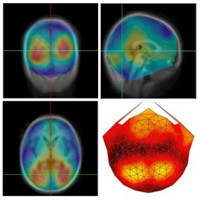
\includegraphics[height=9em]{img/fesi-2014.jpg}}

%%%%%%%%%%%%%%%%%%%%%%%%%%%%%%%%%%%%%%%%%%%%%%%%%%%%%%%%%%%%%%%%%%%%%%%%%%%%%%
%%% Now define the boxes that make up the poster
%%%---------------------------------------------------------------------------
%%% Each box has a name and can be placed absolutely or relatively.
%%% The only inconvenience is that you can only specify a relative position
%%% towards an already declared box. So if you have a box attached to the
%%% bottom, one to the top and a third one which should be in between, you
%%% have to specify the top and bottom boxes before you specify the middle
%%% box.
%%%%%%%%%%%%%%%%%%%%%%%%%%%%%%%%%%%%%%%%%%%%%%%%%%%%%%%%%%%%
%
%%%%%%%%%%%%%%%%%%%%%%%%%%%%%%%%%%%%%%%%%%%%%%%%%%%%%%%%%%%%%%%%%%%%%%%%%%%%%%
\headerbox{Background}{name=bg,column=0,span=1,row=0}
%%%%%%%%%%%%%%%%%%%%%%%%%%%%%%%%%%%%%%%%%%%%%%%%%%%%%%%%%%%%%%%%%%%%%%%%%%%%%%
    {
      \smaller There are many questions about humans being the most intelligent species. Scientists used to believe that humans have a billion neurons in their brain, and that humans had the highest number of neurons than any other species. This was, of course, proven false by Herculano-Houtzel \cite{herculano-houzel-2015}. Her paper shows that the number of neurons for humans according to their brain mass is similar to other species. In fact, animals such as Elephants are outliers. We were curious to analyze the data ourselves and see if we get the same result. Additionally, we tried to find new information from the shared data. The data shared had to be reformatted to perform smooth statistical analyses \cite{Rstudio}. Therefore, datasharing and codesharing issues are also addressed with this research.
    }
%%%%%%%%%%%%%%%%%%%%%%%%%%%%%%%%%%%%%%%%%%%%%%%%%%%%%%%%%%%%%%%%%%%%%%%%%%%%%%
\headerbox{Procedure}{name=method,column=0,span = 1,below=bg}
%%%%%%%%%%%%%%%%%%%%%%%%%%%%%%%%%%%%%%%%%%%%%%%%%%%%%%%%%%%%%%%%%%%%%%%%%%%%%%
    {
\linespread{1.3} \smaller The link for the data was provided with the paper itself, and it was extremely easy to download the raw data-file. The data-file was in an Excel file with different excel sheets dedicated to different areas of the brain. We used 'Rstudio' software \cite{Rstudio} provided by The Pennsylvania State University to manipulate the data. The tasks performed for the 'cleaning' process of the data were as follows:\textsuperscript{1}

\noindent 1. Excel file was converted to a CSV file (Comma Separated Value).

\noindent 2. Empty spaces and extra characters such as '+/-' were removed.

\noindent 3. Each column and variables were renamed.

\noindent 4. Separate column called Brain\_area was created to collapse different sheets of data in one CSV file.

\linespread{5cm} \indent A new Rmarkdown document was created to analyze the data by creating different types of graphs.\textsuperscript{1} The figures provided in the original paper were also recreated. One such example is presented in Figure 2A (recreated graph) and 2B (original graph). The purpose of recreating the graphs was to determine if the data was reproducible. Some of the graphs that were used for analyses showed similar data trends as discussed in the paper. However, Figure 1 showed a new result that was not discussed in the paper.

\scriptsize \linespread{1}
\noindent \textsuperscript{1}All the codes and figures (pdf and png format) produced for this project are openly shared on \url{https://github.com/gilmore-lab/brain-behavior-data}
    }

%%%%%%%%%%%%%%%%%%%%%%%%%%%%%%%%%%%%%%%%%%%%%%%%%%%%%%%%%%%%%%%%%%%%%%%%%%%%%%
  \headerbox{Results: Figure 2A and 2B}{name=res2, column=0, span=1, below=method}
%%%%%%%%%%%%%%%%%%%%%%%%%%%%%%%%%%%%%%%%%%%%%%%%%%%%%%%%%%%%%%%%%%%%%%%%%%%%%%
    {
      \smaller \noindent Fig. 2A shows the three plots that were recreated from \cite{herculano-houzel-2015}. It shows the reproducibility of the data and its figures. Fig. 2B shows the original graphs printed in the article \cite{herculano-houzel-2015}. This graph is labelled 'Fig 3' in the paper.\\
       \textbf{Graph \textit{a}:} Shows a linear relationship between number of neurons and structure mass of Cerebral Cortex without using mouse and naked mole rat as the data with 95\% confidence interval (see Discussion for more detail).
       \textbf{Graph \textit{b}:} Shows a better fit for 95\% confidence interval, but mouse in included in this graph. The naked mole rat is still excluded. The confidence interval changes a little with the inclusion of the mouse which is seen clearly in Fig. 2B than 2A. Here, code sharing would have been useful to recreate the exact plots presented in the paper.
       \textbf{Graph \textit{c}:} Elephant is clearly an outlier, because the number of cerebellar neurons and the cerebral cortex neurons across all species is linear (except for Elephants).
    }

%%%%%%%%%%%%%%%%%%%%%%%%%%%%%%%%%%%%%%%%%%%%%%%%%%%%%%%%%%%%%%%%%%%%%%%%%%%%%%
\headerbox{Figure 1. Self-Analysis Figures}{name=fig1, column=1, span=2, row=0}
%%%%%%%%%%%%%%%%%%%%%%%%%%%%%%%%%%%%%%%%%%%%%%%%%%%%%%%%%%%%%%%%%%%%%%%%%%%%%%
    {
\begin{center}
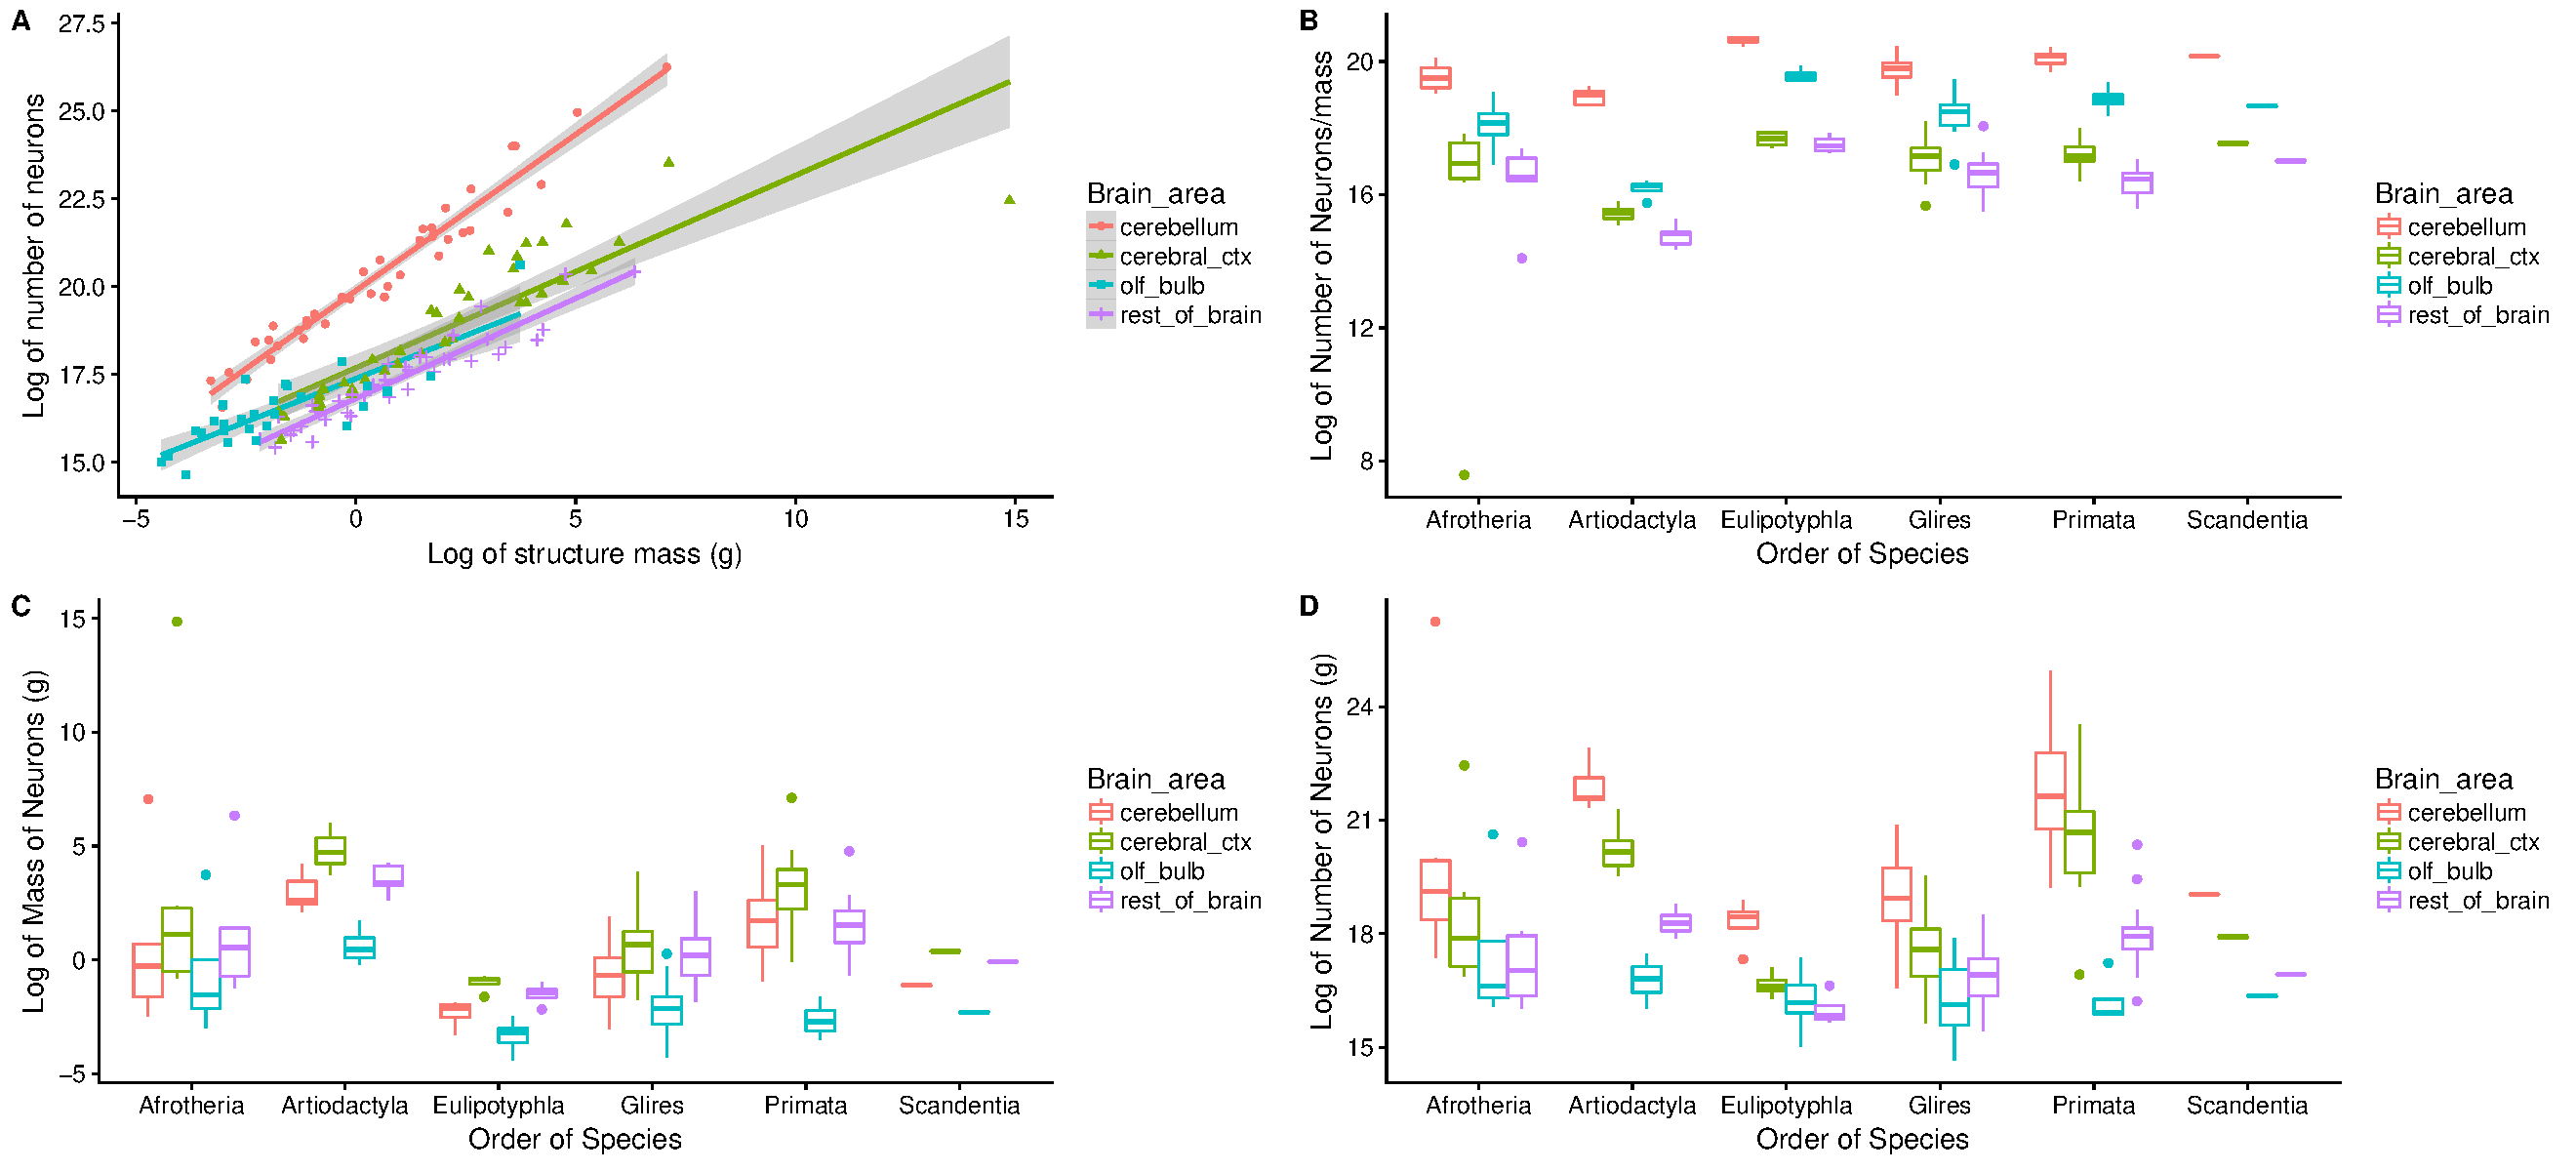
\includegraphics[width = 16cm, height = 9cm]{img/AllPlot.pdf}
%scale=0.36
\smaller 
\end{center}
    }
%%%%%%%%%%%%%%%%%%%%%%%%%%%%%%%%%%%%%%%%%%%%%%%%%%%%%%%%%%%%%%%%%%%%%%%%%%%%%%
\headerbox{Figure 2a. Recreated}{name=fig2a, column=1, span= 1, below = fig1, above=bottom}
%%%%%%%%%%%%%%%%%%%%%%%%%%%%%%%%%%%%%%%%%%%%%%%%%%%%%%%%%%%%%%%%%%%%%%%%%%%%%%
    {
\textbf a

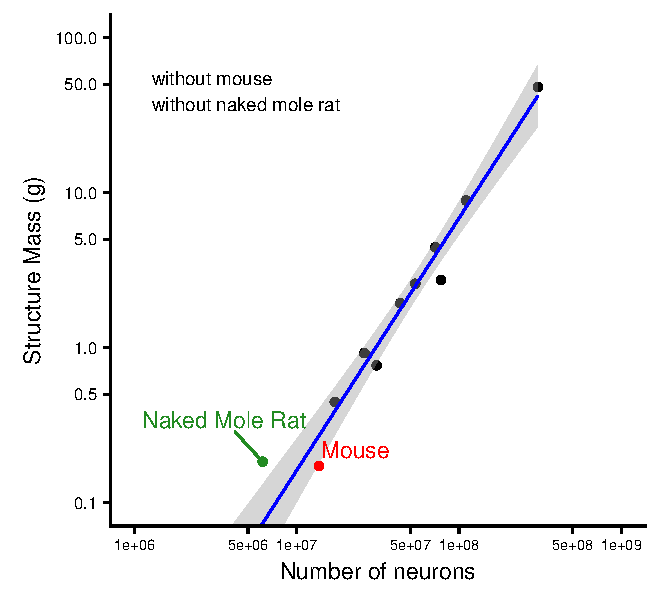
\includegraphics[scale=0.55]{img/no_mouse_nmr.pdf}

\textbf b

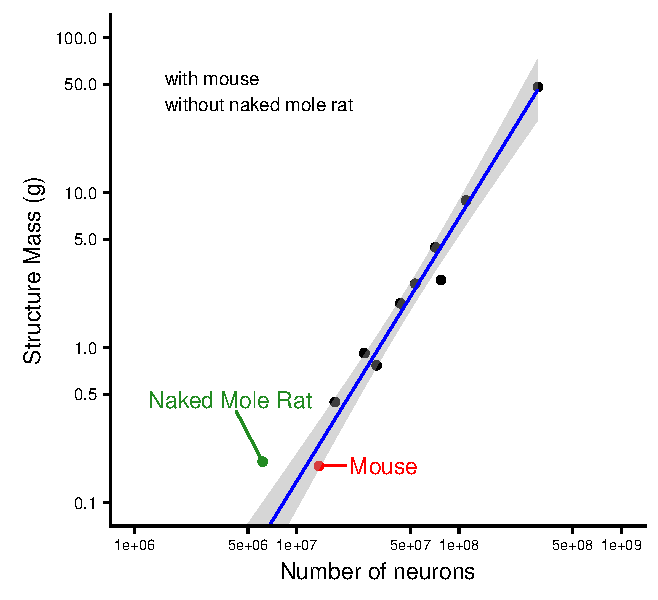
\includegraphics[scale=0.55]{img/nmr_no.pdf}

\textbf c

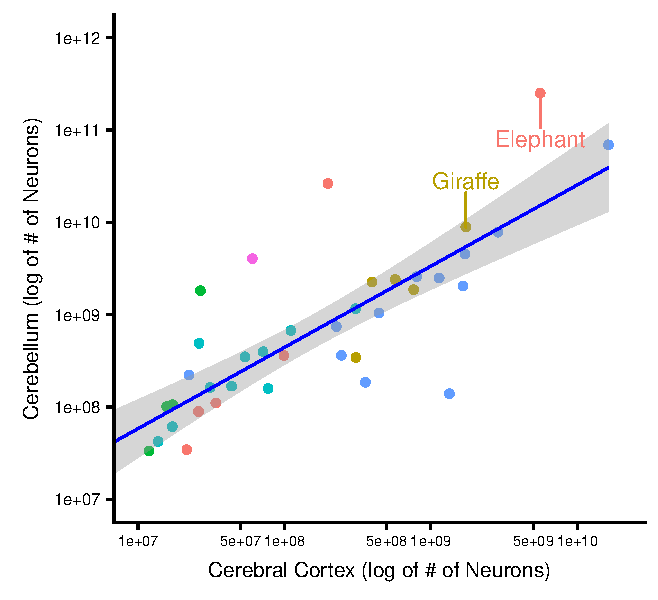
\includegraphics[scale=0.55]{img/cereb_vs_ctx.pdf}
}
%%%%%%%%%%%%%%%%%%%%%%%%%%%%%%%%%%%%%%%%%%%%%%%%%%%%%%%%%%%%%%%%%%%%%%%%%%%%%%
\headerbox{Figure 2b. Original}{name=fig2b, column=2, span= 1, below = fig1, above = bottom}
%%%%%%%%%%%%%%%%%%%%%%%%%%%%%%%%%%%%%%%%%%%%%%%%%%%%%%%%%%%%%%%%%%%%%%%%%%%%%%
    {


\noindent 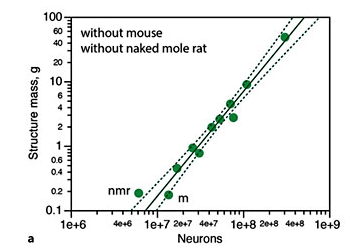
\includegraphics[scale=0.61]{img/HHPlot1.png}
\\
\\
\\
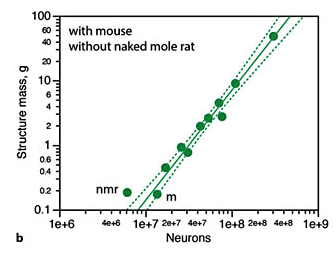
\includegraphics[scale=0.61]{img/HHPlot2.png}
\\
\\
\\
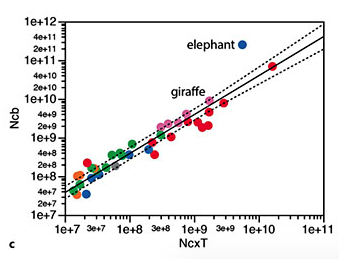
\includegraphics[scale=0.61]{img/HHPlot3.png}
}
%%%%%%%%%%%%%%%%%%%%%%%%%%%%%%%%%%%%%%%%%%%%%%%%%%%%%%%%%%%%%%%%%%%%%%%%%%%%%%
\headerbox{Results: Figure 1}{name=res1, column=3, span=1, row=0}
%%%%%%%%%%%%%%%%%%%%%%%%%%%%%%%%%%%%%%%%%%%%%%%%%%%%%%%%%%%%%%%%%%%%%%%%%%%%%%
    {
    \smaller
    \noindent \textbf{Afrotheria:} belong to the African continent (e.g. golden moles). \textbf{Artiodactyla:} hoofed animals (e.g. Deer). \textbf{Eulipotyphla:} examples are moles and hedgehogs. \textbf{Glires:} include \textit{rodents} (e.g. Rats) and \textit{lagomorphs} (e.g. Rabbits). \textbf{ Primata:} include primates (e.g. gorillas and human beings). \textbf{Scandetia:} include species like \textit{treeshrews}.
    \par \noindent \textbf{(A)} Figure A shows the number of neurons (NoN) per mass of each brain area of all the species. Cerebellum seems to have higher density neurons per mass than cerebral cortex which was discussed in the paper. \\
    \noindent \textbf{(B)} Density of each brain area (NoN/mass) of different Order of Species (OS) is shown here. Trends of individual brain areas seem consistent among different OS. Density of each brain area from highest to lowest are: Cerebellum, Olfactory Bulb (Olf), Cerebral Cortex (Ctx), and Rest of Brain (RoB). \textit{Graph (A)} shows ctx having more density than olf which contradicts  \textit{Graph (B)}. Finally, density of Eulipotyphla seem higher than Primata. \\
    \noindent \textbf{(C)} This graph only looks at the mass of neurons of each brain area arranged by the OS. This graph also shows consistency among different OS. The rank from largest mass to the lowest is: Cerebral Cortex, RoB, Cerebellum, and Olfactory Bulb. Additionally, Artiodactlya show higher mass than Primata. \\
    \noindent \textbf{(D)} This graph solely looks at the NoN on each brain area arranged by the OS. This graph does not show consistency among different OS. NoN from highest to lowest are: Cerebellum, Cerebral Cortex, RoB, and Olfactory Bulb (Eulipotyphla is an exception). Overall, Primata seems have equal NoN to that of Artiodactyla, but Primata has greater variation than Artiodactyla.
}



%%%%%%%%%%%%%%%%%%%%%%%%%%%%%%%%%%%%%%%%%%%%%%%%%%%%%%%%%%%%%%%%%%%%%%%%%%%%%%%
   \headerbox{Discussion}{name=Dis, column=3, below = res1}
%%%%%%%%%%%%%%%%%%%%%%%%%%%%%%%%%%%%%%%%%%%%%%%%%%%%%%%%%%%%%%%%%%%%%%%%%%%%%%%
    {
       \smaller Addressing the issue of reproducible data, researchers should keep in mind about sharing their data in an easily manipulable format. Herculano-Houtzel has shared all her data along with her paper which is extremely helpful for other researchers to perform their personal analyses. However, the format she shared the data was in excel file which was not easily manipulable. As seen in the procedure section, data-cleaning was an essential task before performing the main statistical analyses. \\
       \indent Differences between Fig. 2A and 2B show that R codes used to create the figures should also be shared. Removing 'mouse' from the dataset still shows 'naked mole rat' as an outlier, therefore the data points of the naked mole rat should be used with caution in comparative studies. Similar conclusion goes for elephants, as shown in \textit{Graph 'c'} of Fig. 2A and 2B. \\
       \indent The contradicting results between figures 1A and 1B can be further analyzed by the sensitivity of functioning between those brain areas. Herculano-Houtzel shows that Primates do have higher number of neurons than other OS (as shown in Fig. 1D). This might mean that the density of each brain area does not matter as much as the NoN. Perhaps comparison of task-based performance and NoN, mass, and its density of brain areas of different species can help in determining if the NoN of each species are more predictable of their performance. This can also help to distinguish if Artiodactyla are actually more intelligent than Primates.
     }

%%%%%%%%%%%%%%%%%%%%%%%%%%%%%%%%%%%%%%%%%%%%%%%%%%%%%%%%%%%%%%%%%%%%%%%%%%%%%%%
   \headerbox{Conclusion}{name=Con, column=3, below = Dis, above = bottom}
%%%%%%%%%%%%%%%%%%%%%%%%%%%%%%%%%%%%%%%%%%%%%%%%%%%%%%%%%%%%%%%%%%%%%%%%%%%%%%%
{
\smaller In conclusion, it can be said that, for the time-being, NoN are considered the most predictable way to measure intelligence across different OS. However, task-based performance of each species and its comparison with different brain areas might lead to a different conclusion in the future. Finally, due to Dr. Herculano-Houtzel's shared data, we could further our statistical analyses which shows the importance of data sharing. Additionally, it shows the importance of sharing R codes. These data could also be used for meta-analysis with task-based performance and maybe their diet preferences as well.
}
%%%%%%%%%%%%%%%%%%%%%%%%%%%%%%%%%%%%%%%%%%%%%%%%%%%%%%%%%%%%%%%%%%%%%%%%%%%%%%
 \headerbox{References}{name=refs, column=0, below=res2, above=bottom}
%%%%%%%%%%%%%%%%%%%%%%%%%%%%%%%%%%%%%%%%%%%%%%%%%%%%%%%%%%%%%%%%%%%%%%%%%%%%%%
  {
  %For use with external .bib file
  \tiny
          \renewcommand{\refname}{\vspace{-0.5em}} % removes "References" canned text.
          \bibliographystyle{IEEEtran}
          \bibliography{IEEEabrv,poster_landscape}
}
\end{poster}
\end{document}